% -*- root: ../thesis.tex -*-
%!TEX root = ../thesis.tex
% ******************************* Thesis Appendix A ****************************
\chapter{Additional work} 
\label{appendix:worshoppapers}
The following work does not fit the storyline of the thesis and is therefore presented here only as a side project.

\section{Adaptive Inducing Points Selection for Gaussian Processes}

Two important questions raised when using the sparse \ac{GPs} presented in Section~\ref{sec:sparsegps} are:
How should the inducing points be located?
How many points does one need to reach a desired level of accuracy?
This work tries to answer these questions by proposing an adaptive algorithm, working in $\mathcal{O}(N)$ time and also valid in an online setting.

Although the algorithm proves to be more efficient than standard methods and to have interesting theoretical properties related to Determinantal Point Processes \cite{Kulesza2012}, it has serious tuning issues.
The parameters regulating the algorithm, how often one adds a point or removes one, are tightly correlated to the kernel hyperparameters.
When optimizing hyperparameters during training, an unstable behavior may lead to picking all points as inducing points or selecting none.
I presented this work in the Continual Learning Workshop of ICML 2020.

\textbf{\underline{Authors:}}\\
Th\'eo Galy-Fajou$^1$, Manfred Opper$^1$\\
\small{$^1$TU Berlin}

\textbf{\underline{Details:}}\\
Type: Workshop article\\
Submitted: June 2020\\
Accepted: July 2020\\
URL: \url{https://drive.google.com/file/d/1IPTUBfY_b2WElTWBIVU4lrbHcXnbTWdB/view}\\
Workshop: Continual Learning (ICML 2020)\\


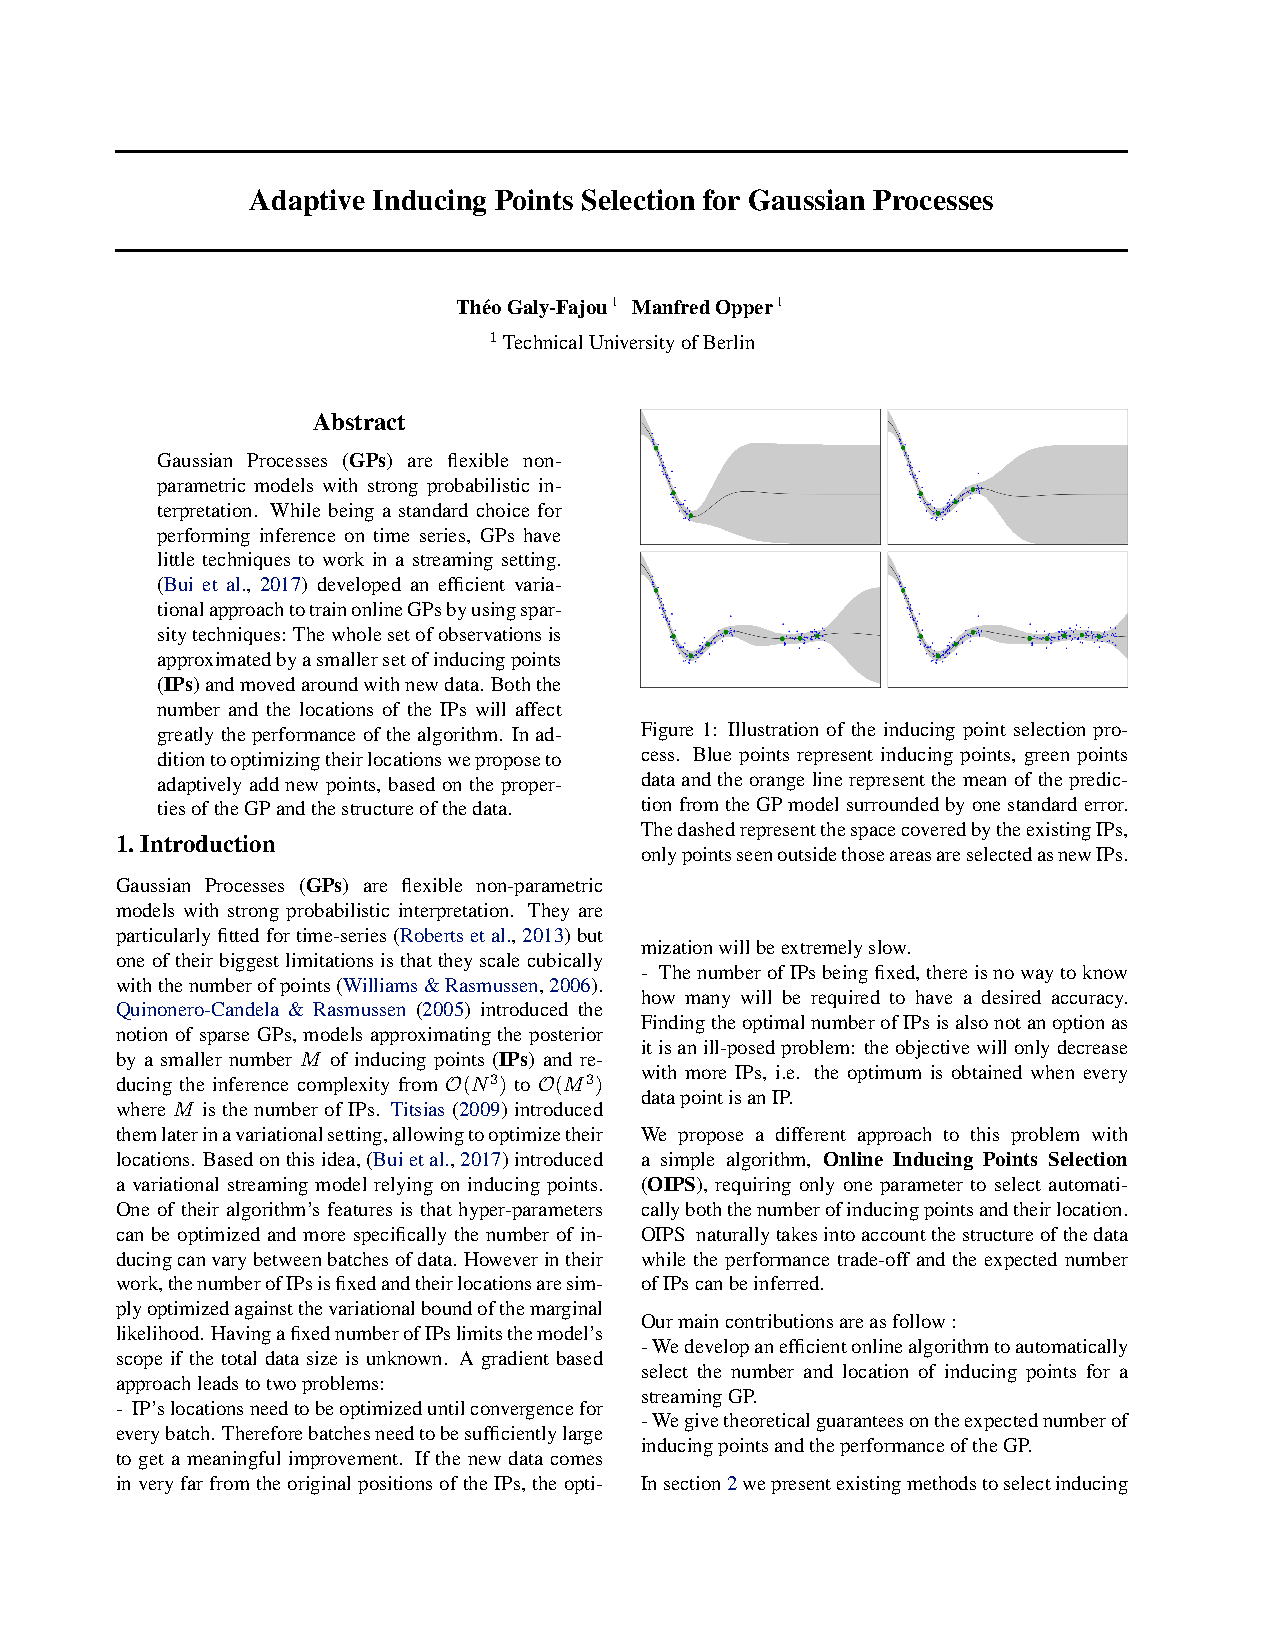
\includepdf[pages=-,pagecommand={},scale=0.95]{./papers/28_CameraReadySubmission_cl_workshop_onlinegp.pdf}

% \section{Evidence Estimation by Kullback-Leibler Integration for Flow-Based Methods}

% \textbf{\underline{Authors:}}\\
% Nikolai Zaki$^1$, Th\'eo Galy-Fajou$^1$, Manfred Opper$^1$\\
% \small{$^1$TU Berlin}

% \textbf{\underline{Details:}}\\
% Type: Workshop article
% Submitted: October 2020\\
% Accepted: December 2020\\
% URL : \url{https://openreview.net/forum?id=LclKtSfmf9I}\\
% Conference: 3rd Symposium on Advances in Approximate Bayesian Inference, 2020\\


% 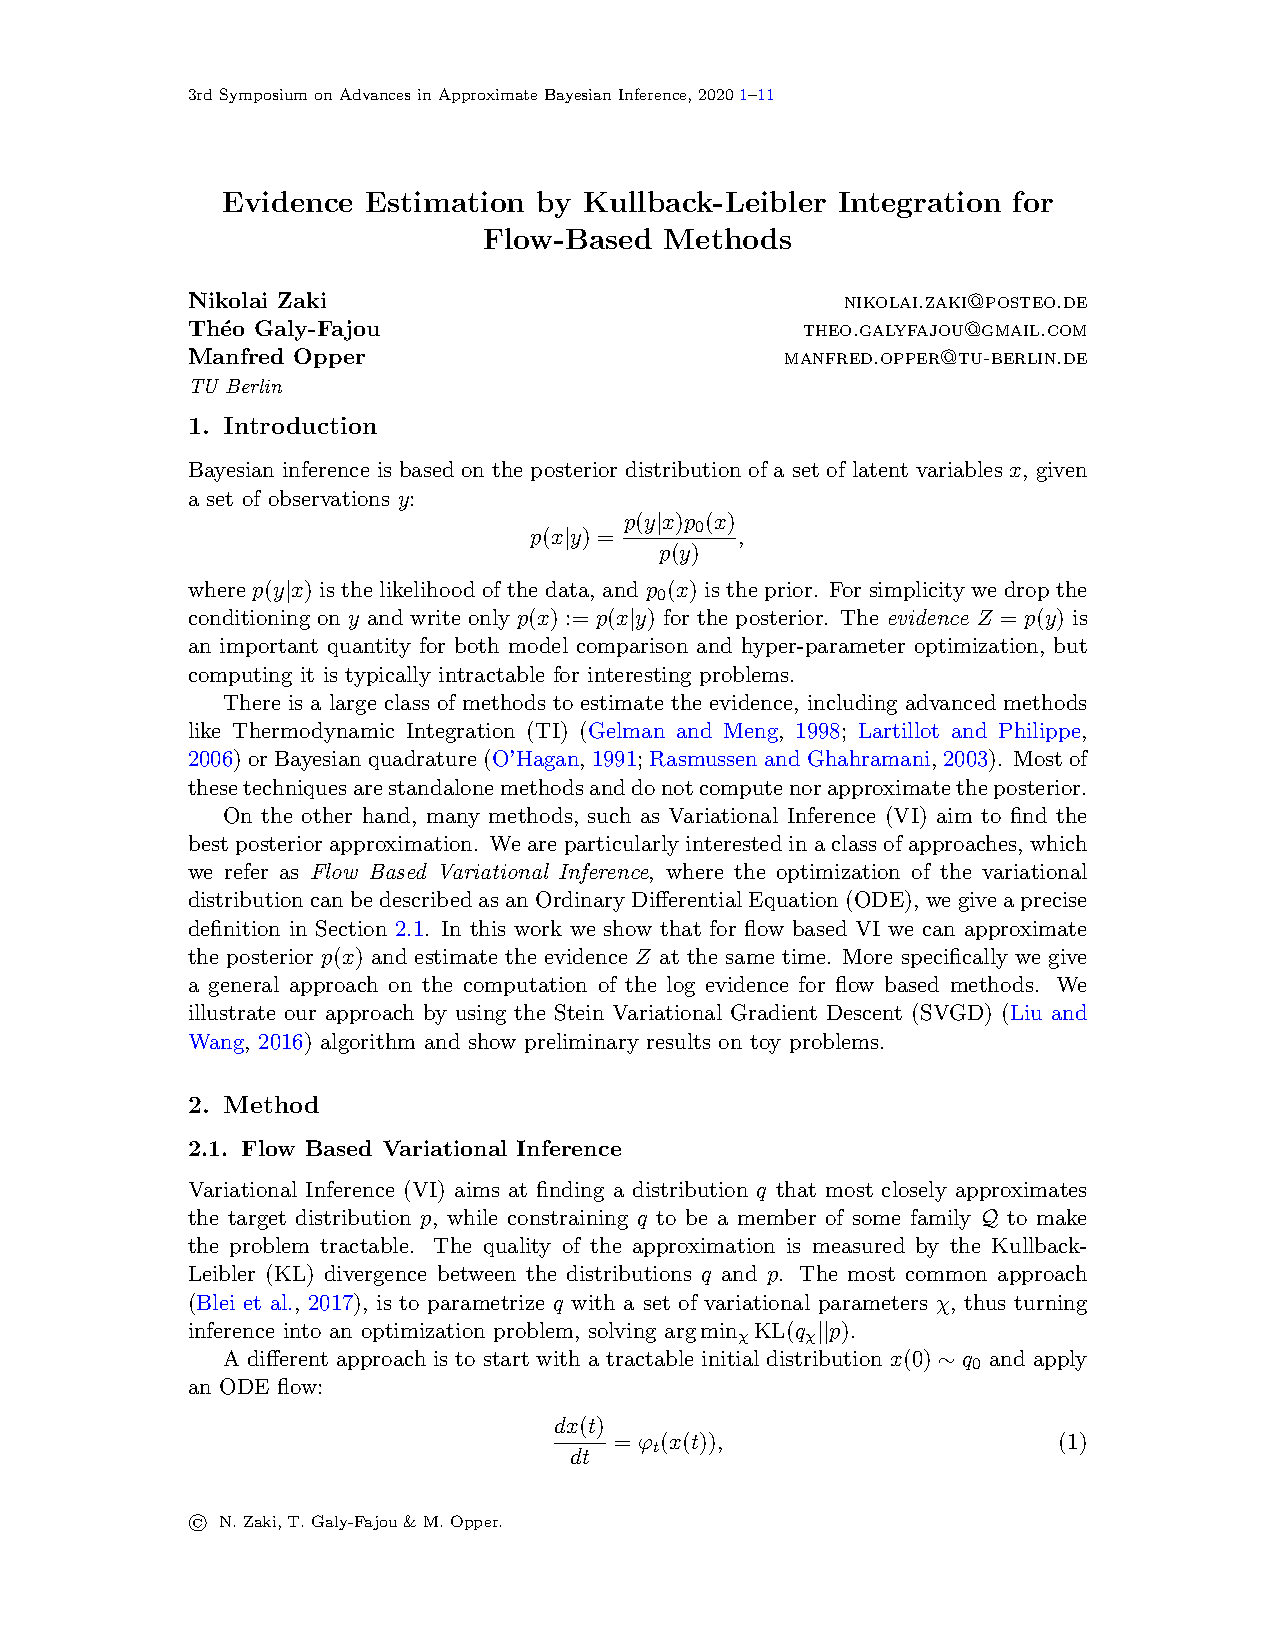
\includepdf[pages=-,pagecommand={},scale=0.95]{./papers/evidence_estimation_by_kullbac.pdf}